% ****************************************************************************************************
% classicthesis-config.tex
% formerly known as loadpackages.sty, classicthesis-ldpkg.sty, and classicthesis-preamble.sty
% Use it at the beginning of your ClassicThesis.tex, or as a LaTeX Preamble
% in your ClassicThesis.{tex,lyx} with % ****************************************************************************************************
% classicthesis-config.tex
% formerly known as loadpackages.sty, classicthesis-ldpkg.sty, and classicthesis-preamble.sty
% Use it at the beginning of your ClassicThesis.tex, or as a LaTeX Preamble
% in your ClassicThesis.{tex,lyx} with % ****************************************************************************************************
% classicthesis-config.tex
% formerly known as loadpackages.sty, classicthesis-ldpkg.sty, and classicthesis-preamble.sty
% Use it at the beginning of your ClassicThesis.tex, or as a LaTeX Preamble
% in your ClassicThesis.{tex,lyx} with % ****************************************************************************************************
% classicthesis-config.tex
% formerly known as loadpackages.sty, classicthesis-ldpkg.sty, and classicthesis-preamble.sty
% Use it at the beginning of your ClassicThesis.tex, or as a LaTeX Preamble
% in your ClassicThesis.{tex,lyx} with \input{classicthesis-config}
% ****************************************************************************************************
% If you like the classicthesis, then I would appreciate a postcard.
% My address can be found in the file ClassicThesis.pdf. A collection
% of the postcards I received so far is available online at
% http://postcards.miede.de
% ****************************************************************************************************


% ****************************************************************************************************
% 0. Set the encoding of your files. UTF-8 is the only sensible encoding nowadays. If you can't read
% äöüßáéçèê∂åëæƒÏ€ then change the encoding setting in your editor, not the line below. If your editor
% does not support utf8 use another editor!
% ****************************************************************************************************
\PassOptionsToPackage{utf8}{inputenc}
  \usepackage{inputenc}

\PassOptionsToPackage{T1}{fontenc} % T2A for cyrillics
  \usepackage{fontenc}


% ****************************************************************************************************
% 1. Configure classicthesis for your needs here, e.g., remove "drafting" below
% in order to deactivate the time-stamp on the pages
% (see ClassicThesis.pdf for more information):
% ****************************************************************************************************
\PassOptionsToPackage{
  drafting=false,    % print version information on the bottom of the pages
  tocaligned=false, % the left column of the toc will be aligned (no indentation)
  dottedtoc=true,  % page numbers in ToC flushed right
  parts,
  eulerchapternumbers=true, % use AMS Euler for chapter font (otherwise Palatino)
  linedheaders=false,       % chaper headers will have line above and beneath
  floatperchapter=true,     % numbering per chapter for all floats (i.e., Figure 1.1)
  eulermath=true,  % use awesome Euler fonts for mathematical formulae (only with pdfLaTeX)
  beramono=true,    % toggle a nice monospaced font (w/ bold)
  subfig,
  palatino=true,    % deactivate standard font for loading another one, see the last section at the end of this file for suggestions
  style=classicthesis % classicthesis, arsclassica
}{classicthesis}


% ****************************************************************************************************
% 2. Personal data and user ad-hoc commands (insert your own data here)
% ****************************************************************************************************
\newcommand{\myTitle}{Deep Learning Methods for Clinical Sleep Analysis\xspace}
\newcommand{\mySubtitle}{An Exploration in Computational Sleep Science}
\newcommand{\myDegree}{Doctor of Philosophy (PhD)\xspace}
\newcommand{\myDocument}{PhD Thesis\xspace}
\newcommand{\myName}{Alexander Neergaard Olesen\xspace}
\newcommand{\myProf}{Associate Professor MSK, Helge. B. D. Sørensen, PhD, MSc. E.E.\xspace}
\newcommand{\myOtherProf}{Professor Poul Jennum, MD, PhD\xspace}
\newcommand{\mySupervisor}{Professor Emmanuel Mignot, MD, PhD\xspace}
\newcommand{\myFaculty}{Department of Health Technology\xspace}
\newcommand{\myDepartment}{Section for Digital Health\xspace}
\newcommand{\myUni}{Technical University of Denmark\xspace}
\newcommand{\myLocation}{Kgs. Lyngby\xspace}
\newcommand{\myTime}{April 2020\xspace}
\newcommand{\myVersion}{\classicthesis}

% ********************************************************************
% Setup, finetuning, and useful commands
% ********************************************************************
\providecommand{\mLyX}{L\kern-.1667em\lower.25em\hbox{Y}\kern-.125emX\@}
\newcommand{\ie}{i.\,e.\xspace}
\newcommand{\Ie}{I.\,e.\xspace}
\newcommand{\eg}{e.\,g.\xspace}
\newcommand{\Eg}{E.\,g.\xspace}
\newcommand{\etc}{\textit{etc.\xspace}}
\newcommand{\etal}{\textit{et al.}\xspace}
% \newcommand{\cohen}{Cohen's $\kappa$}
\newcommand{\wake}{\textsc{w}\xspace}
\newcommand{\rem}{\textsc{r}\xspace}
\newcommand{\nrem}{\textsc{nrem}\xspace}
\newcommand{\nI}{\textsc{n1}\xspace}
\newcommand{\nII}{\textsc{n2}\xspace}
\newcommand{\nIII}{\textsc{n3}\xspace}
\newcommand{\ntI}{\textsc{nt1}\xspace}
\newcommand{\real}[1]{\mathbb{R}^{#1}\xspace}
\newcommand{\cohen}{Cohen's~\ensuremath{\kappa}\xspace}
\newcommand{\ci}[4]{\ensuremath{#1 \pm #2}, \SI{95}{\percent} CI: \ensuremath{\left[ #3-#4 \right]}\xspace}
\newcommand{\muci}[3]{#1 (\SI{95}{\percent} CI: \ensuremath{\left[ #2-#3 \right])}\xspace}
\newcommand{\meanstdrange}[4]{\num[separate-uncertainty]{#1 +- #2} \ensuremath{\left[#3-#4 \right]}\xspace}
\newcommand{\plusminus}[2]{\num[separate-uncertainty]{#1+-#2}}
\newcommand{\train}{\textsc{train}\xspace}
\newcommand{\eval}{\textsc{eval}\xspace}
\newcommand{\test}{\textsc{test}\xspace}
\newcommand{\eog}{\textsc{eog}\xspace}
\newcommand{\mbl}{\mathcal{M}_{\mathrm{FM}}\xspace}
\newcommand{\mpt}{\mathcal{M}_{\mathrm{PT}}\xspace}
\newcommand{\mft}{\mathcal{M}_{\mathrm{FT}}\xspace}
\newcommand{\mse}{\mathcal{M}_{\mathrm{SE}}\xspace}
\newcommand{\N}{\mathbb{N}\xspace}
\newcommand{\hla}{\textsc{hla-dqb1*06:02}\xspace}
\newcommand{\oned}{\textsc{1d}\xspace}
\newcommand{\twod}{\textsc{2d}\xspace}
\newcommand{\threed}{\textsc{3d}\xspace}
\newcommand{\describe}[1]{\acs{#1}:~\acl{#1}}
\newcommand{\R}[1]{\mathbb{R}^{#1}\xspace}
% ****************************************************************************************************


% ****************************************************************************************************
% 3. Loading some handy packages
% ****************************************************************************************************
% ********************************************************************
% Packages with options that might require adjustments
% ********************************************************************
\PassOptionsToPackage{danish,main=english}{babel} % change this to your language(s), main language last
% Spanish languages need extra options in order to work with this template
%\PassOptionsToPackage{spanish,es-lcroman}{babel}
    \usepackage{babel}
\usepackage{epigraph}
\usepackage{csquotes}
\PassOptionsToPackage{%
  backend=biber,bibencoding=utf8, %instead of bibtex
%   backend=bibtex8,bibencoding=ascii,%
  language=auto,%
  style=ieee,%
%   bibstyle=authoryear-comp,
  %style=authoryear-comp, % Author 1999, 2010
  %bibstyle=authoryear,dashed=false, % dashed: substitute rep. author with ---
  sorting=none, % name, year, title
  maxbibnames=99, % default: 3, et al.
  minbibnames=1,
  maxcitenames=3,
  mincitenames=1,
  %backref=true,%
  natbib=true % natbib compatibility mode (\citep and \citet still work)
}{biblatex}
    \usepackage{biblatex}
    
\renewbibmacro{in:}{}
% \renewcommand*{\mkbibnamefamily}[1]{%
%   \ifitemannotation{jointfirst}
%     {#1\(^{\ast}\)}
%     {#1}}

\renewcommand*{\mkbibnamegiven}[1]{%
  \ifitemannotation{highlight}
    {\textbf{#1}}
    {#1}}

\renewcommand*{\mkbibnamefamily}[1]{%
  \ifitemannotation{highlight}
    {\textbf{#1}}
    {#1}}

% \PassOptionsToPackage{fleqn}{amsmath}       % math environments and more by the AMS
%   \usepackage{amsmath}
\PassOptionsToPackage{fleqn}{mathtools}       % math environments and more by the AMS
  \usepackage{mathtools}
\DeclarePairedDelimiter\parentheses{\lparen}{\rparen}
\DeclarePairedDelimiter\abs{\lvert}{\rvert}
% \DeclarePairedDelimiter\abs{\left|}{\left|}
\DeclareMathOperator*{\argmax}{arg\,max}
\DeclareMathOperator*{\argmin}{arg\,min}
\DeclareMathOperator{\sign}{sign}
\newcommand{\func}[2]{\ensuremath{#1 \parentheses*{ #2 }}}
% \newcommand{\parenthesis}[1]{\left( #1 \right)}
\let\originalleft\left
\let\originalright\right
\renewcommand{\left}{\mathopen{}\mathclose\bgroup\originalleft}
\renewcommand{\right}{\aftergroup\egroup\originalright}
\DeclarePairedDelimiter\braces{\lbrace}{\rbrace}
\DeclarePairedDelimiter\brackets{\lbrack}{\rbrack}
\DeclarePairedDelimiter\bbrackets{\llbracket}{\rrbracket}
\DeclareMathOperator{\E}{E}
\DeclareMathOperator{\Var}{Var}
\newcommand{\expect}[1]{\ensuremath{\E\brackets*{#1}}}
\newcommand{\variance}[1]{\ensuremath{\Var\brackets*{#1}}}

% ********************************************************************
% General useful packages
% ********************************************************************
\usepackage{graphicx} %
\graphicspath{ {images/} }
\usepackage{scrhack} % fix warnings when using KOMA with listings package
\usepackage{xspace} % to get the spacing after macros right
\usepackage{relsize}
% \PassOptionsToPackage{printonlyused,smaller}{acronym}
\PassOptionsToPackage{printonlyused}{acronym}
  \usepackage{acronym} % nice macros for handling all acronyms in the thesis
  %\renewcommand{\bflabel}[1]{{#1}\hfill} % fix the list of acronyms --> no longer working
%   \renewcommand*{\acsfont}[1]{\textbf{#1}}
  %\renewcommand*{\aclabelfont}[1]{\acsfont{#1}}
  %\def\bflabel#1{{#1\hfill}}
  \def\bflabel#1{{\acsfont{#1}\hfill}}
  \def\aclabelfont#1{\acsfont{#1}}
\makeatletter
\patchcmd{\AC@@acro}{] #3}{] \MakeUppercase #3}{}{}
\patchcmd{\AC@@acro}{] #3}{] \MakeUppercase #3}{}{}
\makeatother
% \usepackage{tocbibind}
\usepackage{layout}
\usepackage{printlen}
\usepackage{tasks}
\usepackage{textcomp}
% ****************************************************************************************************
%\usepackage{pgfplots} % External TikZ/PGF support (thanks to Andreas Nautsch)
%\usetikzlibrary{external}
%\tikzexternalize[mode=list and make, prefix=ext-tikz/]
% ****************************************************************************************************


% ****************************************************************************************************
% 4. Setup floats: tables, (sub)figures, and captions
% ****************************************************************************************************
\usepackage{tabularx} % better tables
  \setlength{\extrarowheight}{3pt} % increase table row height
\newcommand{\tableheadline}[1]{\multicolumn{1}{l}{\spacedlowsmallcaps{#1}}}
\newcommand{\myfloatalign}{\centering} % to be used with each float for alignment
\usepackage{subfig}
\usepackage{multirow}
\usepackage[flushleft]{threeparttable}
\usepackage{pdflscape}
\usepackage[strict]{changepage}% <-- new
\usepackage{geometry}
% \usepackage{rotation}
% \usepackage{addmargin}

% This length is useful for wider figures and tables
\newlength{\widelength}
\addtolength{\widelength}{\textwidth}
\addtolength{\widelength}{\marginparwidth}
\addtolength{\widelength}{\marginparsep}
\newlength{\marginwidth}
\addtolength{\marginwidth}{\marginparwidth}
\addtolength{\marginwidth}{\marginparsep}


% ****************************************************************************************************


% ****************************************************************************************************
% 5. Setup code listings
% ****************************************************************************************************
\usepackage{listings}
%\lstset{emph={trueIndex,root},emphstyle=\color{BlueViolet}}%\underbar} % for special keywords
\lstset{language=[LaTeX]Tex,%C++,
  morekeywords={PassOptionsToPackage,selectlanguage},
  keywordstyle=\color{RoyalBlue},%\bfseries,
  basicstyle=\small\ttfamily,
  %identifierstyle=\color{NavyBlue},
  commentstyle=\color{Green}\ttfamily,
  stringstyle=\rmfamily,
  numbers=none,%left,%
  numberstyle=\scriptsize,%\tiny
  stepnumber=5,
  numbersep=8pt,
  showstringspaces=false,
  breaklines=true,
  %frameround=ftff,
  %frame=single,
  belowcaptionskip=.75\baselineskip
  %frame=L
}
% ****************************************************************************************************




% ****************************************************************************************************
% 6. Last calls before the bar closes
% ****************************************************************************************************
\usepackage[mode=text]{siunitx}
% \sisetup{detect-all,mode=text}
\usepackage{nth}
% \PassOptionsToPackage{table}{xcolor}
%     \usepackage{xcolor}
% ********************************************************************
% Her Majesty herself
% ********************************************************************
\usepackage{classicthesis}



%%%%%%%%%%%%%%%%%%%%%%%
% Color (Re-Definition)
%%%%%%%%%%%%%%%%%%%%%%%
% according to http://is.gd/aOVVy
\definecolor{dtu-red}{cmyk}{0,.91,.72,.23}
\definecolor{dtu-gray}{cmyk}{0,0,0,.20}
\definecolor{dtu-black}{cmyk}{.20, .20, 0, 1.00}
\definecolor{dtu-navy}{cmyk}{1.00,0.9, 0, 0.6}
\definecolor{CTtitle}{named}{dtu-red}
\definecolor{CTsemi}{named}{dtu-red}
\definecolor{CTurl}{named}{dtu-red}
\definecolor{CTlink}{named}{dtu-black}
\definecolor{CTcitation}{named}{dtu-navy}
\definecolor{lightlightgray}{gray}{0.9}
\definecolor{dtu-link}{RGB}{147,183,209} % define unibe-color for links (Pantone 543, RGB 147,183,209)
\definecolor{dtu-citation}{RGB}{216,140,2} % define unibe-color for citations (Pantone 138, RGB 216,140,2)


% ********************************************************************
% Fine-tune hyperreferences (hyperref should be called last)
% ********************************************************************
\hypersetup{%
  %draft, % hyperref's draft mode, for printing see below
  colorlinks=true, linktocpage=true, pdfstartpage=3, pdfstartview=FitV,%
  % uncomment the following line if you want to have black links (e.g., for printing)
  %colorlinks=false, linktocpage=false, pdfstartpage=3, pdfstartview=FitV, pdfborder={0 0 0},%
  breaklinks=true, pageanchor=true,%
  pdfpagemode=UseNone, %
  % pdfpagemode=UseOutlines,%
  pdfstartpage=1, %
  plainpages=false, bookmarksnumbered, bookmarksopen=true, bookmarksopenlevel=1,%
  hypertexnames=true, pdfhighlight=/O,%nesting=true,%frenchlinks,%
  %urlcolor=dtu-red, %linkcolor=dtu-red, citecolor=dtu-navy, %pagecolor=RoyalBlue,%
  %urlcolor=Black, linkcolor=Black, citecolor=Black, %pagecolor=Black,%
  pdftitle={\myTitle},%
  pdfauthor={\myName, \myUni, \myFaculty},%
  pdfsubject={},%
  pdfkeywords={},%
  pdfcreator={pdfLaTeX},%
  pdfproducer={LaTeX with hyperref and classicthesis}%
}


% ********************************************************************
% Setup autoreferences (hyperref and babel)
% ********************************************************************
% There are some issues regarding autorefnames
% http://www.tex.ac.uk/cgi-bin/texfaq2html?label=latexwords
% you have to redefine the macros for the
% language you use, e.g., american, ngerman
% (as chosen when loading babel/AtBeginDocument)
% ********************************************************************
\makeatletter
\@ifpackageloaded{babel}%
  {%
    \addto\extrasamerican{%
      \renewcommand*{\figureautorefname}{Figure}%
      \renewcommand*{\tableautorefname}{Table}%
      \renewcommand*{\partautorefname}{Part}%
      \renewcommand*{\chapterautorefname}{Chapter}%
      \renewcommand*{\sectionautorefname}{Section}%
      \renewcommand*{\subsectionautorefname}{Section}%
      \renewcommand*{\subsubsectionautorefname}{Section}%
    }%
    \addto\extrasngerman{%
      \renewcommand*{\paragraphautorefname}{Absatz}%
      \renewcommand*{\subparagraphautorefname}{Unterabsatz}%
      \renewcommand*{\footnoteautorefname}{Fu\"snote}%
      \renewcommand*{\FancyVerbLineautorefname}{Zeile}%
      \renewcommand*{\theoremautorefname}{Theorem}%
      \renewcommand*{\appendixautorefname}{Anhang}%
      \renewcommand*{\equationautorefname}{Gleichung}%
      \renewcommand*{\itemautorefname}{Punkt}%
    }%
      % Fix to getting autorefs for subfigures right (thanks to Belinda Vogt for changing the definition)
      \providecommand{\subfigureautorefname}{\figureautorefname}%
    }{\relax}
\makeatother


% ********************************************************************
% Development Stuff
% ********************************************************************
\listfiles
%\PassOptionsToPackage{l2tabu,orthodox,abort}{nag}
%  \usepackage{nag}
%\PassOptionsToPackage{warning, all}{onlyamsmath}
%  \usepackage{onlyamsmath}


% ****************************************************************************************************
% 7. Further adjustments (experimental)
% ****************************************************************************************************
% ********************************************************************
% Changing the text area
% ********************************************************************
%\areaset[current]{312pt}{761pt} % 686 (factor 2.2) + 33 head + 42 head \the\footskip
%\setlength{\marginparwidth}{7em}%
%\setlength{\marginparsep}{2em}%
\captionsetup{format=plain,font=small,labelfont=bf}

% ********************************************************************
% Using different fonts
% ********************************************************************
\usepackage{helvet}
%\usepackage[oldstylenums]{kpfonts} % oldstyle notextcomp
% \usepackage[osf]{libertine}
% \usepackage[light,condensed,math]{iwona}
%\renewcommand{\sfdefault}{iwona}
%\usepackage{lmodern} % <-- no osf support :-(
%\usepackage{cfr-lm} %
%\usepackage[urw-garamond]{mathdesign} <-- no osf support :-(
%\usepackage[default,osfigures]{opensans} % scale=0.95
%\usepackage[sfdefault]{FiraSans}
% \usepackage[opticals,mathlf]{MinionPro} % onlytext
% ********************************************************************
% \usepackage[largesc,osf]{newpxtext}
%\linespread{1.05} % a bit more for Palatino
% Used to fix these:
% https://bitbucket.org/amiede/classicthesis/issues/139/italics-in-pallatino-capitals-chapter
% https://bitbucket.org/amiede/classicthesis/issues/45/problema-testatine-su-classicthesis-style
% ********************************************************************
% ****************************************************************************************************

\usepackage[capitalize,noabbrev]{cleveref}
\usepackage[inline]{enumitem}
\usepackage{todonotes}
\usepackage{stmaryrd}
\usepackage{xfrac}
\usepackage{pdfpages}
\usepackage[version=4]{mhchem}
\usepackage{tcolorbox}

\newcommand{\objective}{to develop a system based on artificial intelligence, that can assist clinicians in the analysis of sleep studies}
\newcommand{\hypothesis}{Advanced biomedical signal processing and machine learning algorithms can be used for efficient, high-performing analysis of sleep studies with regards to}
\newcommand{\hypothesisSleepStages}{Sleep stages can be effectively classified using advanced biomedical signal processing and machine learning algorithms}
\newcommand{\hypothesisSleepEvents}{Sleep events can be precisely annotated using advanced biomedical signal processing and machine learning algorithms}
\newcommand{\hypothesisSleepDisorders}{Sleep disorders can be efficiently diagnosed using advanced biomedical signal processing and machine learning algorithms}
% ****************************************************************************************************
% If you like the classicthesis, then I would appreciate a postcard.
% My address can be found in the file ClassicThesis.pdf. A collection
% of the postcards I received so far is available online at
% http://postcards.miede.de
% ****************************************************************************************************


% ****************************************************************************************************
% 0. Set the encoding of your files. UTF-8 is the only sensible encoding nowadays. If you can't read
% äöüßáéçèê∂åëæƒÏ€ then change the encoding setting in your editor, not the line below. If your editor
% does not support utf8 use another editor!
% ****************************************************************************************************
\PassOptionsToPackage{utf8}{inputenc}
  \usepackage{inputenc}

\PassOptionsToPackage{T1}{fontenc} % T2A for cyrillics
  \usepackage{fontenc}


% ****************************************************************************************************
% 1. Configure classicthesis for your needs here, e.g., remove "drafting" below
% in order to deactivate the time-stamp on the pages
% (see ClassicThesis.pdf for more information):
% ****************************************************************************************************
\PassOptionsToPackage{
  drafting=false,    % print version information on the bottom of the pages
  tocaligned=false, % the left column of the toc will be aligned (no indentation)
  dottedtoc=true,  % page numbers in ToC flushed right
  parts,
  eulerchapternumbers=true, % use AMS Euler for chapter font (otherwise Palatino)
  linedheaders=false,       % chaper headers will have line above and beneath
  floatperchapter=true,     % numbering per chapter for all floats (i.e., Figure 1.1)
  eulermath=true,  % use awesome Euler fonts for mathematical formulae (only with pdfLaTeX)
  beramono=true,    % toggle a nice monospaced font (w/ bold)
  subfig,
  palatino=true,    % deactivate standard font for loading another one, see the last section at the end of this file for suggestions
  style=classicthesis % classicthesis, arsclassica
}{classicthesis}


% ****************************************************************************************************
% 2. Personal data and user ad-hoc commands (insert your own data here)
% ****************************************************************************************************
\newcommand{\myTitle}{Deep Learning Methods for Clinical Sleep Analysis\xspace}
\newcommand{\mySubtitle}{An Exploration in Computational Sleep Science}
\newcommand{\myDegree}{Doctor of Philosophy (PhD)\xspace}
\newcommand{\myDocument}{PhD Thesis\xspace}
\newcommand{\myName}{Alexander Neergaard Olesen\xspace}
\newcommand{\myProf}{Associate Professor MSK, Helge. B. D. Sørensen, PhD, MSc. E.E.\xspace}
\newcommand{\myOtherProf}{Professor Poul Jennum, MD, PhD\xspace}
\newcommand{\mySupervisor}{Professor Emmanuel Mignot, MD, PhD\xspace}
\newcommand{\myFaculty}{Department of Health Technology\xspace}
\newcommand{\myDepartment}{Section for Digital Health\xspace}
\newcommand{\myUni}{Technical University of Denmark\xspace}
\newcommand{\myLocation}{Kgs. Lyngby\xspace}
\newcommand{\myTime}{April 2020\xspace}
\newcommand{\myVersion}{\classicthesis}

% ********************************************************************
% Setup, finetuning, and useful commands
% ********************************************************************
\providecommand{\mLyX}{L\kern-.1667em\lower.25em\hbox{Y}\kern-.125emX\@}
\newcommand{\ie}{i.\,e.\xspace}
\newcommand{\Ie}{I.\,e.\xspace}
\newcommand{\eg}{e.\,g.\xspace}
\newcommand{\Eg}{E.\,g.\xspace}
\newcommand{\etc}{\textit{etc.\xspace}}
\newcommand{\etal}{\textit{et al.}\xspace}
% \newcommand{\cohen}{Cohen's $\kappa$}
\newcommand{\wake}{\textsc{w}\xspace}
\newcommand{\rem}{\textsc{r}\xspace}
\newcommand{\nrem}{\textsc{nrem}\xspace}
\newcommand{\nI}{\textsc{n1}\xspace}
\newcommand{\nII}{\textsc{n2}\xspace}
\newcommand{\nIII}{\textsc{n3}\xspace}
\newcommand{\ntI}{\textsc{nt1}\xspace}
\newcommand{\real}[1]{\mathbb{R}^{#1}\xspace}
\newcommand{\cohen}{Cohen's~\ensuremath{\kappa}\xspace}
\newcommand{\ci}[4]{\ensuremath{#1 \pm #2}, \SI{95}{\percent} CI: \ensuremath{\left[ #3-#4 \right]}\xspace}
\newcommand{\muci}[3]{#1 (\SI{95}{\percent} CI: \ensuremath{\left[ #2-#3 \right])}\xspace}
\newcommand{\meanstdrange}[4]{\num[separate-uncertainty]{#1 +- #2} \ensuremath{\left[#3-#4 \right]}\xspace}
\newcommand{\plusminus}[2]{\num[separate-uncertainty]{#1+-#2}}
\newcommand{\train}{\textsc{train}\xspace}
\newcommand{\eval}{\textsc{eval}\xspace}
\newcommand{\test}{\textsc{test}\xspace}
\newcommand{\eog}{\textsc{eog}\xspace}
\newcommand{\mbl}{\mathcal{M}_{\mathrm{FM}}\xspace}
\newcommand{\mpt}{\mathcal{M}_{\mathrm{PT}}\xspace}
\newcommand{\mft}{\mathcal{M}_{\mathrm{FT}}\xspace}
\newcommand{\mse}{\mathcal{M}_{\mathrm{SE}}\xspace}
\newcommand{\N}{\mathbb{N}\xspace}
\newcommand{\hla}{\textsc{hla-dqb1*06:02}\xspace}
\newcommand{\oned}{\textsc{1d}\xspace}
\newcommand{\twod}{\textsc{2d}\xspace}
\newcommand{\threed}{\textsc{3d}\xspace}
\newcommand{\describe}[1]{\acs{#1}:~\acl{#1}}
\newcommand{\R}[1]{\mathbb{R}^{#1}\xspace}
% ****************************************************************************************************


% ****************************************************************************************************
% 3. Loading some handy packages
% ****************************************************************************************************
% ********************************************************************
% Packages with options that might require adjustments
% ********************************************************************
\PassOptionsToPackage{danish,main=english}{babel} % change this to your language(s), main language last
% Spanish languages need extra options in order to work with this template
%\PassOptionsToPackage{spanish,es-lcroman}{babel}
    \usepackage{babel}
\usepackage{epigraph}
\usepackage{csquotes}
\PassOptionsToPackage{%
  backend=biber,bibencoding=utf8, %instead of bibtex
%   backend=bibtex8,bibencoding=ascii,%
  language=auto,%
  style=ieee,%
%   bibstyle=authoryear-comp,
  %style=authoryear-comp, % Author 1999, 2010
  %bibstyle=authoryear,dashed=false, % dashed: substitute rep. author with ---
  sorting=none, % name, year, title
  maxbibnames=99, % default: 3, et al.
  minbibnames=1,
  maxcitenames=3,
  mincitenames=1,
  %backref=true,%
  natbib=true % natbib compatibility mode (\citep and \citet still work)
}{biblatex}
    \usepackage{biblatex}
    
\renewbibmacro{in:}{}
% \renewcommand*{\mkbibnamefamily}[1]{%
%   \ifitemannotation{jointfirst}
%     {#1\(^{\ast}\)}
%     {#1}}

\renewcommand*{\mkbibnamegiven}[1]{%
  \ifitemannotation{highlight}
    {\textbf{#1}}
    {#1}}

\renewcommand*{\mkbibnamefamily}[1]{%
  \ifitemannotation{highlight}
    {\textbf{#1}}
    {#1}}

% \PassOptionsToPackage{fleqn}{amsmath}       % math environments and more by the AMS
%   \usepackage{amsmath}
\PassOptionsToPackage{fleqn}{mathtools}       % math environments and more by the AMS
  \usepackage{mathtools}
\DeclarePairedDelimiter\parentheses{\lparen}{\rparen}
\DeclarePairedDelimiter\abs{\lvert}{\rvert}
% \DeclarePairedDelimiter\abs{\left|}{\left|}
\DeclareMathOperator*{\argmax}{arg\,max}
\DeclareMathOperator*{\argmin}{arg\,min}
\DeclareMathOperator{\sign}{sign}
\newcommand{\func}[2]{\ensuremath{#1 \parentheses*{ #2 }}}
% \newcommand{\parenthesis}[1]{\left( #1 \right)}
\let\originalleft\left
\let\originalright\right
\renewcommand{\left}{\mathopen{}\mathclose\bgroup\originalleft}
\renewcommand{\right}{\aftergroup\egroup\originalright}
\DeclarePairedDelimiter\braces{\lbrace}{\rbrace}
\DeclarePairedDelimiter\brackets{\lbrack}{\rbrack}
\DeclarePairedDelimiter\bbrackets{\llbracket}{\rrbracket}
\DeclareMathOperator{\E}{E}
\DeclareMathOperator{\Var}{Var}
\newcommand{\expect}[1]{\ensuremath{\E\brackets*{#1}}}
\newcommand{\variance}[1]{\ensuremath{\Var\brackets*{#1}}}

% ********************************************************************
% General useful packages
% ********************************************************************
\usepackage{graphicx} %
\graphicspath{ {images/} }
\usepackage{scrhack} % fix warnings when using KOMA with listings package
\usepackage{xspace} % to get the spacing after macros right
\usepackage{relsize}
% \PassOptionsToPackage{printonlyused,smaller}{acronym}
\PassOptionsToPackage{printonlyused}{acronym}
  \usepackage{acronym} % nice macros for handling all acronyms in the thesis
  %\renewcommand{\bflabel}[1]{{#1}\hfill} % fix the list of acronyms --> no longer working
%   \renewcommand*{\acsfont}[1]{\textbf{#1}}
  %\renewcommand*{\aclabelfont}[1]{\acsfont{#1}}
  %\def\bflabel#1{{#1\hfill}}
  \def\bflabel#1{{\acsfont{#1}\hfill}}
  \def\aclabelfont#1{\acsfont{#1}}
\makeatletter
\patchcmd{\AC@@acro}{] #3}{] \MakeUppercase #3}{}{}
\patchcmd{\AC@@acro}{] #3}{] \MakeUppercase #3}{}{}
\makeatother
% \usepackage{tocbibind}
\usepackage{layout}
\usepackage{printlen}
\usepackage{tasks}
\usepackage{textcomp}
% ****************************************************************************************************
%\usepackage{pgfplots} % External TikZ/PGF support (thanks to Andreas Nautsch)
%\usetikzlibrary{external}
%\tikzexternalize[mode=list and make, prefix=ext-tikz/]
% ****************************************************************************************************


% ****************************************************************************************************
% 4. Setup floats: tables, (sub)figures, and captions
% ****************************************************************************************************
\usepackage{tabularx} % better tables
  \setlength{\extrarowheight}{3pt} % increase table row height
\newcommand{\tableheadline}[1]{\multicolumn{1}{l}{\spacedlowsmallcaps{#1}}}
\newcommand{\myfloatalign}{\centering} % to be used with each float for alignment
\usepackage{subfig}
\usepackage{multirow}
\usepackage[flushleft]{threeparttable}
\usepackage{pdflscape}
\usepackage[strict]{changepage}% <-- new
\usepackage{geometry}
% \usepackage{rotation}
% \usepackage{addmargin}

% This length is useful for wider figures and tables
\newlength{\widelength}
\addtolength{\widelength}{\textwidth}
\addtolength{\widelength}{\marginparwidth}
\addtolength{\widelength}{\marginparsep}
\newlength{\marginwidth}
\addtolength{\marginwidth}{\marginparwidth}
\addtolength{\marginwidth}{\marginparsep}


% ****************************************************************************************************


% ****************************************************************************************************
% 5. Setup code listings
% ****************************************************************************************************
\usepackage{listings}
%\lstset{emph={trueIndex,root},emphstyle=\color{BlueViolet}}%\underbar} % for special keywords
\lstset{language=[LaTeX]Tex,%C++,
  morekeywords={PassOptionsToPackage,selectlanguage},
  keywordstyle=\color{RoyalBlue},%\bfseries,
  basicstyle=\small\ttfamily,
  %identifierstyle=\color{NavyBlue},
  commentstyle=\color{Green}\ttfamily,
  stringstyle=\rmfamily,
  numbers=none,%left,%
  numberstyle=\scriptsize,%\tiny
  stepnumber=5,
  numbersep=8pt,
  showstringspaces=false,
  breaklines=true,
  %frameround=ftff,
  %frame=single,
  belowcaptionskip=.75\baselineskip
  %frame=L
}
% ****************************************************************************************************




% ****************************************************************************************************
% 6. Last calls before the bar closes
% ****************************************************************************************************
\usepackage[mode=text]{siunitx}
% \sisetup{detect-all,mode=text}
\usepackage{nth}
% \PassOptionsToPackage{table}{xcolor}
%     \usepackage{xcolor}
% ********************************************************************
% Her Majesty herself
% ********************************************************************
\usepackage{classicthesis}



%%%%%%%%%%%%%%%%%%%%%%%
% Color (Re-Definition)
%%%%%%%%%%%%%%%%%%%%%%%
% according to http://is.gd/aOVVy
\definecolor{dtu-red}{cmyk}{0,.91,.72,.23}
\definecolor{dtu-gray}{cmyk}{0,0,0,.20}
\definecolor{dtu-black}{cmyk}{.20, .20, 0, 1.00}
\definecolor{dtu-navy}{cmyk}{1.00,0.9, 0, 0.6}
\definecolor{CTtitle}{named}{dtu-red}
\definecolor{CTsemi}{named}{dtu-red}
\definecolor{CTurl}{named}{dtu-red}
\definecolor{CTlink}{named}{dtu-black}
\definecolor{CTcitation}{named}{dtu-navy}
\definecolor{lightlightgray}{gray}{0.9}
\definecolor{dtu-link}{RGB}{147,183,209} % define unibe-color for links (Pantone 543, RGB 147,183,209)
\definecolor{dtu-citation}{RGB}{216,140,2} % define unibe-color for citations (Pantone 138, RGB 216,140,2)


% ********************************************************************
% Fine-tune hyperreferences (hyperref should be called last)
% ********************************************************************
\hypersetup{%
  %draft, % hyperref's draft mode, for printing see below
  colorlinks=true, linktocpage=true, pdfstartpage=3, pdfstartview=FitV,%
  % uncomment the following line if you want to have black links (e.g., for printing)
  %colorlinks=false, linktocpage=false, pdfstartpage=3, pdfstartview=FitV, pdfborder={0 0 0},%
  breaklinks=true, pageanchor=true,%
  pdfpagemode=UseNone, %
  % pdfpagemode=UseOutlines,%
  pdfstartpage=1, %
  plainpages=false, bookmarksnumbered, bookmarksopen=true, bookmarksopenlevel=1,%
  hypertexnames=true, pdfhighlight=/O,%nesting=true,%frenchlinks,%
  %urlcolor=dtu-red, %linkcolor=dtu-red, citecolor=dtu-navy, %pagecolor=RoyalBlue,%
  %urlcolor=Black, linkcolor=Black, citecolor=Black, %pagecolor=Black,%
  pdftitle={\myTitle},%
  pdfauthor={\myName, \myUni, \myFaculty},%
  pdfsubject={},%
  pdfkeywords={},%
  pdfcreator={pdfLaTeX},%
  pdfproducer={LaTeX with hyperref and classicthesis}%
}


% ********************************************************************
% Setup autoreferences (hyperref and babel)
% ********************************************************************
% There are some issues regarding autorefnames
% http://www.tex.ac.uk/cgi-bin/texfaq2html?label=latexwords
% you have to redefine the macros for the
% language you use, e.g., american, ngerman
% (as chosen when loading babel/AtBeginDocument)
% ********************************************************************
\makeatletter
\@ifpackageloaded{babel}%
  {%
    \addto\extrasamerican{%
      \renewcommand*{\figureautorefname}{Figure}%
      \renewcommand*{\tableautorefname}{Table}%
      \renewcommand*{\partautorefname}{Part}%
      \renewcommand*{\chapterautorefname}{Chapter}%
      \renewcommand*{\sectionautorefname}{Section}%
      \renewcommand*{\subsectionautorefname}{Section}%
      \renewcommand*{\subsubsectionautorefname}{Section}%
    }%
    \addto\extrasngerman{%
      \renewcommand*{\paragraphautorefname}{Absatz}%
      \renewcommand*{\subparagraphautorefname}{Unterabsatz}%
      \renewcommand*{\footnoteautorefname}{Fu\"snote}%
      \renewcommand*{\FancyVerbLineautorefname}{Zeile}%
      \renewcommand*{\theoremautorefname}{Theorem}%
      \renewcommand*{\appendixautorefname}{Anhang}%
      \renewcommand*{\equationautorefname}{Gleichung}%
      \renewcommand*{\itemautorefname}{Punkt}%
    }%
      % Fix to getting autorefs for subfigures right (thanks to Belinda Vogt for changing the definition)
      \providecommand{\subfigureautorefname}{\figureautorefname}%
    }{\relax}
\makeatother


% ********************************************************************
% Development Stuff
% ********************************************************************
\listfiles
%\PassOptionsToPackage{l2tabu,orthodox,abort}{nag}
%  \usepackage{nag}
%\PassOptionsToPackage{warning, all}{onlyamsmath}
%  \usepackage{onlyamsmath}


% ****************************************************************************************************
% 7. Further adjustments (experimental)
% ****************************************************************************************************
% ********************************************************************
% Changing the text area
% ********************************************************************
%\areaset[current]{312pt}{761pt} % 686 (factor 2.2) + 33 head + 42 head \the\footskip
%\setlength{\marginparwidth}{7em}%
%\setlength{\marginparsep}{2em}%
\captionsetup{format=plain,font=small,labelfont=bf}

% ********************************************************************
% Using different fonts
% ********************************************************************
\usepackage{helvet}
%\usepackage[oldstylenums]{kpfonts} % oldstyle notextcomp
% \usepackage[osf]{libertine}
% \usepackage[light,condensed,math]{iwona}
%\renewcommand{\sfdefault}{iwona}
%\usepackage{lmodern} % <-- no osf support :-(
%\usepackage{cfr-lm} %
%\usepackage[urw-garamond]{mathdesign} <-- no osf support :-(
%\usepackage[default,osfigures]{opensans} % scale=0.95
%\usepackage[sfdefault]{FiraSans}
% \usepackage[opticals,mathlf]{MinionPro} % onlytext
% ********************************************************************
% \usepackage[largesc,osf]{newpxtext}
%\linespread{1.05} % a bit more for Palatino
% Used to fix these:
% https://bitbucket.org/amiede/classicthesis/issues/139/italics-in-pallatino-capitals-chapter
% https://bitbucket.org/amiede/classicthesis/issues/45/problema-testatine-su-classicthesis-style
% ********************************************************************
% ****************************************************************************************************

\usepackage[capitalize,noabbrev]{cleveref}
\usepackage[inline]{enumitem}
\usepackage{todonotes}
\usepackage{stmaryrd}
\usepackage{xfrac}
\usepackage{pdfpages}
\usepackage[version=4]{mhchem}
\usepackage{tcolorbox}

\newcommand{\objective}{to develop a system based on artificial intelligence, that can assist clinicians in the analysis of sleep studies}
\newcommand{\hypothesis}{Advanced biomedical signal processing and machine learning algorithms can be used for efficient, high-performing analysis of sleep studies with regards to}
\newcommand{\hypothesisSleepStages}{Sleep stages can be effectively classified using advanced biomedical signal processing and machine learning algorithms}
\newcommand{\hypothesisSleepEvents}{Sleep events can be precisely annotated using advanced biomedical signal processing and machine learning algorithms}
\newcommand{\hypothesisSleepDisorders}{Sleep disorders can be efficiently diagnosed using advanced biomedical signal processing and machine learning algorithms}
% ****************************************************************************************************
% If you like the classicthesis, then I would appreciate a postcard.
% My address can be found in the file ClassicThesis.pdf. A collection
% of the postcards I received so far is available online at
% http://postcards.miede.de
% ****************************************************************************************************


% ****************************************************************************************************
% 0. Set the encoding of your files. UTF-8 is the only sensible encoding nowadays. If you can't read
% äöüßáéçèê∂åëæƒÏ€ then change the encoding setting in your editor, not the line below. If your editor
% does not support utf8 use another editor!
% ****************************************************************************************************
\PassOptionsToPackage{utf8}{inputenc}
  \usepackage{inputenc}

\PassOptionsToPackage{T1}{fontenc} % T2A for cyrillics
  \usepackage{fontenc}


% ****************************************************************************************************
% 1. Configure classicthesis for your needs here, e.g., remove "drafting" below
% in order to deactivate the time-stamp on the pages
% (see ClassicThesis.pdf for more information):
% ****************************************************************************************************
\PassOptionsToPackage{
  drafting=false,    % print version information on the bottom of the pages
  tocaligned=false, % the left column of the toc will be aligned (no indentation)
  dottedtoc=true,  % page numbers in ToC flushed right
  parts,
  eulerchapternumbers=true, % use AMS Euler for chapter font (otherwise Palatino)
  linedheaders=false,       % chaper headers will have line above and beneath
  floatperchapter=true,     % numbering per chapter for all floats (i.e., Figure 1.1)
  eulermath=true,  % use awesome Euler fonts for mathematical formulae (only with pdfLaTeX)
  beramono=true,    % toggle a nice monospaced font (w/ bold)
  subfig,
  palatino=true,    % deactivate standard font for loading another one, see the last section at the end of this file for suggestions
  style=classicthesis % classicthesis, arsclassica
}{classicthesis}


% ****************************************************************************************************
% 2. Personal data and user ad-hoc commands (insert your own data here)
% ****************************************************************************************************
\newcommand{\myTitle}{Deep Learning Methods for Clinical Sleep Analysis\xspace}
\newcommand{\mySubtitle}{An Exploration in Computational Sleep Science}
\newcommand{\myDegree}{Doctor of Philosophy (PhD)\xspace}
\newcommand{\myDocument}{PhD Thesis\xspace}
\newcommand{\myName}{Alexander Neergaard Olesen\xspace}
\newcommand{\myProf}{Associate Professor MSK, Helge. B. D. Sørensen, PhD, MSc. E.E.\xspace}
\newcommand{\myOtherProf}{Professor Poul Jennum, MD, PhD\xspace}
\newcommand{\mySupervisor}{Professor Emmanuel Mignot, MD, PhD\xspace}
\newcommand{\myFaculty}{Department of Health Technology\xspace}
\newcommand{\myDepartment}{Section for Digital Health\xspace}
\newcommand{\myUni}{Technical University of Denmark\xspace}
\newcommand{\myLocation}{Kgs. Lyngby\xspace}
\newcommand{\myTime}{April 2020\xspace}
\newcommand{\myVersion}{\classicthesis}

% ********************************************************************
% Setup, finetuning, and useful commands
% ********************************************************************
\providecommand{\mLyX}{L\kern-.1667em\lower.25em\hbox{Y}\kern-.125emX\@}
\newcommand{\ie}{i.\,e.\xspace}
\newcommand{\Ie}{I.\,e.\xspace}
\newcommand{\eg}{e.\,g.\xspace}
\newcommand{\Eg}{E.\,g.\xspace}
\newcommand{\etc}{\textit{etc.\xspace}}
\newcommand{\etal}{\textit{et al.}\xspace}
% \newcommand{\cohen}{Cohen's $\kappa$}
\newcommand{\wake}{\textsc{w}\xspace}
\newcommand{\rem}{\textsc{r}\xspace}
\newcommand{\nrem}{\textsc{nrem}\xspace}
\newcommand{\nI}{\textsc{n1}\xspace}
\newcommand{\nII}{\textsc{n2}\xspace}
\newcommand{\nIII}{\textsc{n3}\xspace}
\newcommand{\ntI}{\textsc{nt1}\xspace}
\newcommand{\real}[1]{\mathbb{R}^{#1}\xspace}
\newcommand{\cohen}{Cohen's~\ensuremath{\kappa}\xspace}
\newcommand{\ci}[4]{\ensuremath{#1 \pm #2}, \SI{95}{\percent} CI: \ensuremath{\left[ #3-#4 \right]}\xspace}
\newcommand{\muci}[3]{#1 (\SI{95}{\percent} CI: \ensuremath{\left[ #2-#3 \right])}\xspace}
\newcommand{\meanstdrange}[4]{\num[separate-uncertainty]{#1 +- #2} \ensuremath{\left[#3-#4 \right]}\xspace}
\newcommand{\plusminus}[2]{\num[separate-uncertainty]{#1+-#2}}
\newcommand{\train}{\textsc{train}\xspace}
\newcommand{\eval}{\textsc{eval}\xspace}
\newcommand{\test}{\textsc{test}\xspace}
\newcommand{\eog}{\textsc{eog}\xspace}
\newcommand{\mbl}{\mathcal{M}_{\mathrm{FM}}\xspace}
\newcommand{\mpt}{\mathcal{M}_{\mathrm{PT}}\xspace}
\newcommand{\mft}{\mathcal{M}_{\mathrm{FT}}\xspace}
\newcommand{\mse}{\mathcal{M}_{\mathrm{SE}}\xspace}
\newcommand{\N}{\mathbb{N}\xspace}
\newcommand{\hla}{\textsc{hla-dqb1*06:02}\xspace}
\newcommand{\oned}{\textsc{1d}\xspace}
\newcommand{\twod}{\textsc{2d}\xspace}
\newcommand{\threed}{\textsc{3d}\xspace}
\newcommand{\describe}[1]{\acs{#1}:~\acl{#1}}
\newcommand{\R}[1]{\mathbb{R}^{#1}\xspace}
% ****************************************************************************************************


% ****************************************************************************************************
% 3. Loading some handy packages
% ****************************************************************************************************
% ********************************************************************
% Packages with options that might require adjustments
% ********************************************************************
\PassOptionsToPackage{danish,main=english}{babel} % change this to your language(s), main language last
% Spanish languages need extra options in order to work with this template
%\PassOptionsToPackage{spanish,es-lcroman}{babel}
    \usepackage{babel}
\usepackage{epigraph}
\usepackage{csquotes}
\PassOptionsToPackage{%
  backend=biber,bibencoding=utf8, %instead of bibtex
%   backend=bibtex8,bibencoding=ascii,%
  language=auto,%
  style=ieee,%
%   bibstyle=authoryear-comp,
  %style=authoryear-comp, % Author 1999, 2010
  %bibstyle=authoryear,dashed=false, % dashed: substitute rep. author with ---
  sorting=none, % name, year, title
  maxbibnames=99, % default: 3, et al.
  minbibnames=1,
  maxcitenames=3,
  mincitenames=1,
  %backref=true,%
  natbib=true % natbib compatibility mode (\citep and \citet still work)
}{biblatex}
    \usepackage{biblatex}
    
\renewbibmacro{in:}{}
% \renewcommand*{\mkbibnamefamily}[1]{%
%   \ifitemannotation{jointfirst}
%     {#1\(^{\ast}\)}
%     {#1}}

\renewcommand*{\mkbibnamegiven}[1]{%
  \ifitemannotation{highlight}
    {\textbf{#1}}
    {#1}}

\renewcommand*{\mkbibnamefamily}[1]{%
  \ifitemannotation{highlight}
    {\textbf{#1}}
    {#1}}

% \PassOptionsToPackage{fleqn}{amsmath}       % math environments and more by the AMS
%   \usepackage{amsmath}
\PassOptionsToPackage{fleqn}{mathtools}       % math environments and more by the AMS
  \usepackage{mathtools}
\DeclarePairedDelimiter\parentheses{\lparen}{\rparen}
\DeclarePairedDelimiter\abs{\lvert}{\rvert}
% \DeclarePairedDelimiter\abs{\left|}{\left|}
\DeclareMathOperator*{\argmax}{arg\,max}
\DeclareMathOperator*{\argmin}{arg\,min}
\DeclareMathOperator{\sign}{sign}
\newcommand{\func}[2]{\ensuremath{#1 \parentheses*{ #2 }}}
% \newcommand{\parenthesis}[1]{\left( #1 \right)}
\let\originalleft\left
\let\originalright\right
\renewcommand{\left}{\mathopen{}\mathclose\bgroup\originalleft}
\renewcommand{\right}{\aftergroup\egroup\originalright}
\DeclarePairedDelimiter\braces{\lbrace}{\rbrace}
\DeclarePairedDelimiter\brackets{\lbrack}{\rbrack}
\DeclarePairedDelimiter\bbrackets{\llbracket}{\rrbracket}
\DeclareMathOperator{\E}{E}
\DeclareMathOperator{\Var}{Var}
\newcommand{\expect}[1]{\ensuremath{\E\brackets*{#1}}}
\newcommand{\variance}[1]{\ensuremath{\Var\brackets*{#1}}}

% ********************************************************************
% General useful packages
% ********************************************************************
\usepackage{graphicx} %
\graphicspath{ {images/} }
\usepackage{scrhack} % fix warnings when using KOMA with listings package
\usepackage{xspace} % to get the spacing after macros right
\usepackage{relsize}
% \PassOptionsToPackage{printonlyused,smaller}{acronym}
\PassOptionsToPackage{printonlyused}{acronym}
  \usepackage{acronym} % nice macros for handling all acronyms in the thesis
  %\renewcommand{\bflabel}[1]{{#1}\hfill} % fix the list of acronyms --> no longer working
%   \renewcommand*{\acsfont}[1]{\textbf{#1}}
  %\renewcommand*{\aclabelfont}[1]{\acsfont{#1}}
  %\def\bflabel#1{{#1\hfill}}
  \def\bflabel#1{{\acsfont{#1}\hfill}}
  \def\aclabelfont#1{\acsfont{#1}}
\makeatletter
\patchcmd{\AC@@acro}{] #3}{] \MakeUppercase #3}{}{}
\patchcmd{\AC@@acro}{] #3}{] \MakeUppercase #3}{}{}
\makeatother
% \usepackage{tocbibind}
\usepackage{layout}
\usepackage{printlen}
\usepackage{tasks}
\usepackage{textcomp}
% ****************************************************************************************************
%\usepackage{pgfplots} % External TikZ/PGF support (thanks to Andreas Nautsch)
%\usetikzlibrary{external}
%\tikzexternalize[mode=list and make, prefix=ext-tikz/]
% ****************************************************************************************************


% ****************************************************************************************************
% 4. Setup floats: tables, (sub)figures, and captions
% ****************************************************************************************************
\usepackage{tabularx} % better tables
  \setlength{\extrarowheight}{3pt} % increase table row height
\newcommand{\tableheadline}[1]{\multicolumn{1}{l}{\spacedlowsmallcaps{#1}}}
\newcommand{\myfloatalign}{\centering} % to be used with each float for alignment
\usepackage{subfig}
\usepackage{multirow}
\usepackage[flushleft]{threeparttable}
\usepackage{pdflscape}
\usepackage[strict]{changepage}% <-- new
\usepackage{geometry}
% \usepackage{rotation}
% \usepackage{addmargin}

% This length is useful for wider figures and tables
\newlength{\widelength}
\addtolength{\widelength}{\textwidth}
\addtolength{\widelength}{\marginparwidth}
\addtolength{\widelength}{\marginparsep}
\newlength{\marginwidth}
\addtolength{\marginwidth}{\marginparwidth}
\addtolength{\marginwidth}{\marginparsep}


% ****************************************************************************************************


% ****************************************************************************************************
% 5. Setup code listings
% ****************************************************************************************************
\usepackage{listings}
%\lstset{emph={trueIndex,root},emphstyle=\color{BlueViolet}}%\underbar} % for special keywords
\lstset{language=[LaTeX]Tex,%C++,
  morekeywords={PassOptionsToPackage,selectlanguage},
  keywordstyle=\color{RoyalBlue},%\bfseries,
  basicstyle=\small\ttfamily,
  %identifierstyle=\color{NavyBlue},
  commentstyle=\color{Green}\ttfamily,
  stringstyle=\rmfamily,
  numbers=none,%left,%
  numberstyle=\scriptsize,%\tiny
  stepnumber=5,
  numbersep=8pt,
  showstringspaces=false,
  breaklines=true,
  %frameround=ftff,
  %frame=single,
  belowcaptionskip=.75\baselineskip
  %frame=L
}
% ****************************************************************************************************




% ****************************************************************************************************
% 6. Last calls before the bar closes
% ****************************************************************************************************
\usepackage[mode=text]{siunitx}
% \sisetup{detect-all,mode=text}
\usepackage{nth}
% \PassOptionsToPackage{table}{xcolor}
%     \usepackage{xcolor}
% ********************************************************************
% Her Majesty herself
% ********************************************************************
\usepackage{classicthesis}



%%%%%%%%%%%%%%%%%%%%%%%
% Color (Re-Definition)
%%%%%%%%%%%%%%%%%%%%%%%
% according to http://is.gd/aOVVy
\definecolor{dtu-red}{cmyk}{0,.91,.72,.23}
\definecolor{dtu-gray}{cmyk}{0,0,0,.20}
\definecolor{dtu-black}{cmyk}{.20, .20, 0, 1.00}
\definecolor{dtu-navy}{cmyk}{1.00,0.9, 0, 0.6}
\definecolor{CTtitle}{named}{dtu-red}
\definecolor{CTsemi}{named}{dtu-red}
\definecolor{CTurl}{named}{dtu-red}
\definecolor{CTlink}{named}{dtu-black}
\definecolor{CTcitation}{named}{dtu-navy}
\definecolor{lightlightgray}{gray}{0.9}
\definecolor{dtu-link}{RGB}{147,183,209} % define unibe-color for links (Pantone 543, RGB 147,183,209)
\definecolor{dtu-citation}{RGB}{216,140,2} % define unibe-color for citations (Pantone 138, RGB 216,140,2)


% ********************************************************************
% Fine-tune hyperreferences (hyperref should be called last)
% ********************************************************************
\hypersetup{%
  %draft, % hyperref's draft mode, for printing see below
  colorlinks=true, linktocpage=true, pdfstartpage=3, pdfstartview=FitV,%
  % uncomment the following line if you want to have black links (e.g., for printing)
  %colorlinks=false, linktocpage=false, pdfstartpage=3, pdfstartview=FitV, pdfborder={0 0 0},%
  breaklinks=true, pageanchor=true,%
  pdfpagemode=UseNone, %
  % pdfpagemode=UseOutlines,%
  pdfstartpage=1, %
  plainpages=false, bookmarksnumbered, bookmarksopen=true, bookmarksopenlevel=1,%
  hypertexnames=true, pdfhighlight=/O,%nesting=true,%frenchlinks,%
  %urlcolor=dtu-red, %linkcolor=dtu-red, citecolor=dtu-navy, %pagecolor=RoyalBlue,%
  %urlcolor=Black, linkcolor=Black, citecolor=Black, %pagecolor=Black,%
  pdftitle={\myTitle},%
  pdfauthor={\myName, \myUni, \myFaculty},%
  pdfsubject={},%
  pdfkeywords={},%
  pdfcreator={pdfLaTeX},%
  pdfproducer={LaTeX with hyperref and classicthesis}%
}


% ********************************************************************
% Setup autoreferences (hyperref and babel)
% ********************************************************************
% There are some issues regarding autorefnames
% http://www.tex.ac.uk/cgi-bin/texfaq2html?label=latexwords
% you have to redefine the macros for the
% language you use, e.g., american, ngerman
% (as chosen when loading babel/AtBeginDocument)
% ********************************************************************
\makeatletter
\@ifpackageloaded{babel}%
  {%
    \addto\extrasamerican{%
      \renewcommand*{\figureautorefname}{Figure}%
      \renewcommand*{\tableautorefname}{Table}%
      \renewcommand*{\partautorefname}{Part}%
      \renewcommand*{\chapterautorefname}{Chapter}%
      \renewcommand*{\sectionautorefname}{Section}%
      \renewcommand*{\subsectionautorefname}{Section}%
      \renewcommand*{\subsubsectionautorefname}{Section}%
    }%
    \addto\extrasngerman{%
      \renewcommand*{\paragraphautorefname}{Absatz}%
      \renewcommand*{\subparagraphautorefname}{Unterabsatz}%
      \renewcommand*{\footnoteautorefname}{Fu\"snote}%
      \renewcommand*{\FancyVerbLineautorefname}{Zeile}%
      \renewcommand*{\theoremautorefname}{Theorem}%
      \renewcommand*{\appendixautorefname}{Anhang}%
      \renewcommand*{\equationautorefname}{Gleichung}%
      \renewcommand*{\itemautorefname}{Punkt}%
    }%
      % Fix to getting autorefs for subfigures right (thanks to Belinda Vogt for changing the definition)
      \providecommand{\subfigureautorefname}{\figureautorefname}%
    }{\relax}
\makeatother


% ********************************************************************
% Development Stuff
% ********************************************************************
\listfiles
%\PassOptionsToPackage{l2tabu,orthodox,abort}{nag}
%  \usepackage{nag}
%\PassOptionsToPackage{warning, all}{onlyamsmath}
%  \usepackage{onlyamsmath}


% ****************************************************************************************************
% 7. Further adjustments (experimental)
% ****************************************************************************************************
% ********************************************************************
% Changing the text area
% ********************************************************************
%\areaset[current]{312pt}{761pt} % 686 (factor 2.2) + 33 head + 42 head \the\footskip
%\setlength{\marginparwidth}{7em}%
%\setlength{\marginparsep}{2em}%
\captionsetup{format=plain,font=small,labelfont=bf}

% ********************************************************************
% Using different fonts
% ********************************************************************
\usepackage{helvet}
%\usepackage[oldstylenums]{kpfonts} % oldstyle notextcomp
% \usepackage[osf]{libertine}
% \usepackage[light,condensed,math]{iwona}
%\renewcommand{\sfdefault}{iwona}
%\usepackage{lmodern} % <-- no osf support :-(
%\usepackage{cfr-lm} %
%\usepackage[urw-garamond]{mathdesign} <-- no osf support :-(
%\usepackage[default,osfigures]{opensans} % scale=0.95
%\usepackage[sfdefault]{FiraSans}
% \usepackage[opticals,mathlf]{MinionPro} % onlytext
% ********************************************************************
% \usepackage[largesc,osf]{newpxtext}
%\linespread{1.05} % a bit more for Palatino
% Used to fix these:
% https://bitbucket.org/amiede/classicthesis/issues/139/italics-in-pallatino-capitals-chapter
% https://bitbucket.org/amiede/classicthesis/issues/45/problema-testatine-su-classicthesis-style
% ********************************************************************
% ****************************************************************************************************

\usepackage[capitalize,noabbrev]{cleveref}
\usepackage[inline]{enumitem}
\usepackage{todonotes}
\usepackage{stmaryrd}
\usepackage{xfrac}
\usepackage{pdfpages}
\usepackage[version=4]{mhchem}
\usepackage{tcolorbox}

\newcommand{\objective}{to develop a system based on artificial intelligence, that can assist clinicians in the analysis of sleep studies}
\newcommand{\hypothesis}{Advanced biomedical signal processing and machine learning algorithms can be used for efficient, high-performing analysis of sleep studies with regards to}
\newcommand{\hypothesisSleepStages}{Sleep stages can be effectively classified using advanced biomedical signal processing and machine learning algorithms}
\newcommand{\hypothesisSleepEvents}{Sleep events can be precisely annotated using advanced biomedical signal processing and machine learning algorithms}
\newcommand{\hypothesisSleepDisorders}{Sleep disorders can be efficiently diagnosed using advanced biomedical signal processing and machine learning algorithms}
% ****************************************************************************************************
% If you like the classicthesis, then I would appreciate a postcard.
% My address can be found in the file ClassicThesis.pdf. A collection
% of the postcards I received so far is available online at
% http://postcards.miede.de
% ****************************************************************************************************


% ****************************************************************************************************
% 0. Set the encoding of your files. UTF-8 is the only sensible encoding nowadays. If you can't read
% äöüßáéçèê∂åëæƒÏ€ then change the encoding setting in your editor, not the line below. If your editor
% does not support utf8 use another editor!
% ****************************************************************************************************
\PassOptionsToPackage{utf8}{inputenc}
  \usepackage{inputenc}

\PassOptionsToPackage{T1}{fontenc} % T2A for cyrillics
  \usepackage{fontenc}


% ****************************************************************************************************
% 1. Configure classicthesis for your needs here, e.g., remove "drafting" below
% in order to deactivate the time-stamp on the pages
% (see ClassicThesis.pdf for more information):
% ****************************************************************************************************
\PassOptionsToPackage{
  drafting=false,    % print version information on the bottom of the pages
  tocaligned=false, % the left column of the toc will be aligned (no indentation)
  dottedtoc=true,  % page numbers in ToC flushed right
  parts,
  eulerchapternumbers=true, % use AMS Euler for chapter font (otherwise Palatino)
  linedheaders=false,       % chaper headers will have line above and beneath
  floatperchapter=true,     % numbering per chapter for all floats (i.e., Figure 1.1)
  eulermath=true,  % use awesome Euler fonts for mathematical formulae (only with pdfLaTeX)
  beramono=true,    % toggle a nice monospaced font (w/ bold)
  subfig,
  palatino=true,    % deactivate standard font for loading another one, see the last section at the end of this file for suggestions
  style=classicthesis % classicthesis, arsclassica
}{classicthesis}


% ****************************************************************************************************
% 2. Personal data and user ad-hoc commands (insert your own data here)
% ****************************************************************************************************
\newcommand{\myTitle}{Deep Learning Methods for Clinical Sleep Analysis\xspace}
\newcommand{\mySubtitle}{An Exploration in Computational Sleep Science}
\newcommand{\myDegree}{Doctor of Philosophy (PhD)\xspace}
\newcommand{\myDocument}{PhD Thesis\xspace}
\newcommand{\myName}{Alexander Neergaard Olesen\xspace}
\newcommand{\myProf}{Associate Professor MSK, Helge. B. D. Sørensen, PhD, MSc. E.E.\xspace}
\newcommand{\myOtherProf}{Professor Poul Jennum, MD, PhD\xspace}
\newcommand{\mySupervisor}{Professor Emmanuel Mignot, MD, PhD\xspace}
\newcommand{\myFaculty}{Department of Health Technology\xspace}
\newcommand{\myDepartment}{Section for Digital Health\xspace}
\newcommand{\myUni}{Technical University of Denmark\xspace}
\newcommand{\myLocation}{Kgs. Lyngby\xspace}
\newcommand{\myTime}{April 2020\xspace}
\newcommand{\myVersion}{\classicthesis}
\newcommand{\myAddress}{Ørsteds Plads\\Building 345C\\DK-2800 \myLocation\\Denmark}

% ********************************************************************
% Setup, finetuning, and useful commands
% ********************************************************************
\providecommand{\mLyX}{L\kern-.1667em\lower.25em\hbox{Y}\kern-.125emX\@}
\newcommand{\ie}{i.\,e.\xspace}
\newcommand{\Ie}{I.\,e.\xspace}
\newcommand{\eg}{e.\,g.\xspace}
\newcommand{\Eg}{E.\,g.\xspace}
\newcommand{\etc}{\textit{etc.\xspace}}
\newcommand{\etal}{\textit{et al.}\xspace}
% \newcommand{\cohen}{Cohen's $\kappa$}
\newcommand{\wake}{\textsc{w}\xspace}
\newcommand{\rem}{\textsc{r}\xspace}
\newcommand{\nrem}{\textsc{nrem}\xspace}
\newcommand{\nI}{\textsc{n1}\xspace}
\newcommand{\nII}{\textsc{n2}\xspace}
\newcommand{\nIII}{\textsc{n3}\xspace}
\newcommand{\ntI}{\textsc{nt1}\xspace}
\newcommand{\real}[1]{\mathbb{R}^{#1}\xspace}
\newcommand{\cohen}{Cohen's~\ensuremath{\kappa}\xspace}
\newcommand{\ci}[4]{\ensuremath{#1 \pm #2}, \SI{95}{\percent} CI: \ensuremath{\left[ #3-#4 \right]}\xspace}
\newcommand{\muci}[3]{#1 (\SI{95}{\percent} CI: \ensuremath{\left[ #2-#3 \right])}\xspace}
\newcommand{\meanstdrange}[4]{\num[separate-uncertainty]{#1 +- #2} \ensuremath{\left[#3-#4 \right]}\xspace}
\newcommand{\plusminus}[2]{\num[separate-uncertainty]{#1+-#2}}
\newcommand{\train}{\textsc{train}\xspace}
\newcommand{\eval}{\textsc{eval}\xspace}
\newcommand{\test}{\textsc{test}\xspace}
\newcommand{\eog}{\textsc{eog}\xspace}
\newcommand{\mbl}{\mathcal{M}_{\mathrm{FM}}\xspace}
\newcommand{\mpt}{\mathcal{M}_{\mathrm{PT}}\xspace}
\newcommand{\mft}{\mathcal{M}_{\mathrm{FT}}\xspace}
\newcommand{\mse}{\mathcal{M}_{\mathrm{SE}}\xspace}
\newcommand{\N}{\mathbb{N}\xspace}
\newcommand{\hla}{\textsc{hla-dqb1*06:02}\xspace}
\newcommand{\oned}{\textsc{1d}\xspace}
\newcommand{\twod}{\textsc{2d}\xspace}
\newcommand{\threed}{\textsc{3d}\xspace}
\newcommand{\describe}[1]{\acs{#1}:~\acl{#1}}
\newcommand{\R}[1]{\mathbb{R}^{#1}\xspace}
% ****************************************************************************************************


% ****************************************************************************************************
% 3. Loading some handy packages
% ****************************************************************************************************
% ********************************************************************
% Packages with options that might require adjustments
% ********************************************************************
\PassOptionsToPackage{danish,main=english}{babel} % change this to your language(s), main language last
% Spanish languages need extra options in order to work with this template
%\PassOptionsToPackage{spanish,es-lcroman}{babel}
    \usepackage{babel}
\usepackage{epigraph}
\usepackage{csquotes}
\PassOptionsToPackage{%
  backend=biber,bibencoding=utf8, %instead of bibtex
%   backend=bibtex8,bibencoding=ascii,%
  language=auto,%
  style=ieee,%
%   bibstyle=authoryear-comp,
  %style=authoryear-comp, % Author 1999, 2010
  %bibstyle=authoryear,dashed=false, % dashed: substitute rep. author with ---
  sorting=none, % name, year, title
  maxbibnames=99, % default: 3, et al.
  minbibnames=1,
  maxcitenames=3,
  mincitenames=1,
  %backref=true,%
  natbib=true % natbib compatibility mode (\citep and \citet still work)
}{biblatex}
    \usepackage{biblatex}
    
\renewbibmacro{in:}{}
% \renewcommand*{\mkbibnamefamily}[1]{%
%   \ifitemannotation{jointfirst}
%     {#1\(^{\ast}\)}
%     {#1}}

\renewcommand*{\mkbibnamegiven}[1]{%
  \ifitemannotation{highlight}
    {\textbf{#1}}
    {#1}}

\renewcommand*{\mkbibnamefamily}[1]{%
  \ifitemannotation{highlight}
    {\textbf{#1}}
    {#1}}

% \PassOptionsToPackage{fleqn}{amsmath}       % math environments and more by the AMS
%   \usepackage{amsmath}
\PassOptionsToPackage{fleqn}{mathtools}       % math environments and more by the AMS
  \usepackage{mathtools}
\DeclarePairedDelimiter\parentheses{\lparen}{\rparen}
\DeclarePairedDelimiter\abs{\lvert}{\rvert}
% \DeclarePairedDelimiter\abs{\left|}{\left|}
\DeclareMathOperator*{\argmax}{arg\,max}
\DeclareMathOperator*{\argmin}{arg\,min}
\DeclareMathOperator{\sign}{sign}
\newcommand{\func}[2]{\ensuremath{#1 \parentheses*{ #2 }}}
% \newcommand{\parenthesis}[1]{\left( #1 \right)}
\let\originalleft\left
\let\originalright\right
\renewcommand{\left}{\mathopen{}\mathclose\bgroup\originalleft}
\renewcommand{\right}{\aftergroup\egroup\originalright}
\DeclarePairedDelimiter\braces{\lbrace}{\rbrace}
\DeclarePairedDelimiter\brackets{\lbrack}{\rbrack}
\DeclarePairedDelimiter\bbrackets{\llbracket}{\rrbracket}
\DeclareMathOperator{\E}{E}
\DeclareMathOperator{\Var}{Var}
\newcommand{\expect}[1]{\ensuremath{\E\brackets*{#1}}}
\newcommand{\variance}[1]{\ensuremath{\Var\brackets*{#1}}}

% ********************************************************************
% General useful packages
% ********************************************************************
\usepackage{graphicx} %
\graphicspath{ {images/} }
\usepackage{scrhack} % fix warnings when using KOMA with listings package
\usepackage{xspace} % to get the spacing after macros right
\usepackage{relsize}
% \PassOptionsToPackage{printonlyused,smaller}{acronym}
\PassOptionsToPackage{printonlyused}{acronym}
  \usepackage{acronym} % nice macros for handling all acronyms in the thesis
  %\renewcommand{\bflabel}[1]{{#1}\hfill} % fix the list of acronyms --> no longer working
%   \renewcommand*{\acsfont}[1]{\textbf{#1}}
  %\renewcommand*{\aclabelfont}[1]{\acsfont{#1}}
  %\def\bflabel#1{{#1\hfill}}
  \def\bflabel#1{{\acsfont{#1}\hfill}}
  \def\aclabelfont#1{\acsfont{#1}}
\makeatletter
\patchcmd{\AC@@acro}{] #3}{] \MakeUppercase #3}{}{}
\patchcmd{\AC@@acro}{] #3}{] \MakeUppercase #3}{}{}
\makeatother
% \usepackage{tocbibind}
\usepackage{layout}
\usepackage{printlen}
\usepackage{tasks}
\usepackage{textcomp}
% ****************************************************************************************************
%\usepackage{pgfplots} % External TikZ/PGF support (thanks to Andreas Nautsch)
%\usetikzlibrary{external}
%\tikzexternalize[mode=list and make, prefix=ext-tikz/]
% ****************************************************************************************************


% ****************************************************************************************************
% 4. Setup floats: tables, (sub)figures, and captions
% ****************************************************************************************************
\usepackage{tabularx} % better tables
  \setlength{\extrarowheight}{3pt} % increase table row height
\newcommand{\tableheadline}[1]{\multicolumn{1}{l}{\spacedlowsmallcaps{#1}}}
\newcommand{\myfloatalign}{\centering} % to be used with each float for alignment
\usepackage{subfig}
\usepackage{multirow}
\usepackage[flushleft]{threeparttable}
\usepackage{pdflscape}
\usepackage[strict]{changepage}% <-- new
\usepackage{geometry}
% \usepackage{rotation}
% \usepackage{addmargin}

% This length is useful for wider figures and tables
\newlength{\widelength}
\addtolength{\widelength}{\textwidth}
\addtolength{\widelength}{\marginparwidth}
\addtolength{\widelength}{\marginparsep}
\newlength{\marginwidth}
\addtolength{\marginwidth}{\marginparwidth}
\addtolength{\marginwidth}{\marginparsep}


% ****************************************************************************************************


% ****************************************************************************************************
% 5. Setup code listings
% ****************************************************************************************************
\usepackage{listings}
%\lstset{emph={trueIndex,root},emphstyle=\color{BlueViolet}}%\underbar} % for special keywords
\lstset{language=[LaTeX]Tex,%C++,
  morekeywords={PassOptionsToPackage,selectlanguage},
  keywordstyle=\color{RoyalBlue},%\bfseries,
  basicstyle=\small\ttfamily,
  %identifierstyle=\color{NavyBlue},
  commentstyle=\color{Green}\ttfamily,
  stringstyle=\rmfamily,
  numbers=none,%left,%
  numberstyle=\scriptsize,%\tiny
  stepnumber=5,
  numbersep=8pt,
  showstringspaces=false,
  breaklines=true,
  %frameround=ftff,
  %frame=single,
  belowcaptionskip=.75\baselineskip
  %frame=L
}
% ****************************************************************************************************




% ****************************************************************************************************
% 6. Last calls before the bar closes
% ****************************************************************************************************
\usepackage[mode=text]{siunitx}
% \sisetup{detect-all,mode=text}
\usepackage{nth}
% \PassOptionsToPackage{table}{xcolor}
%     \usepackage{xcolor}
% ********************************************************************
% Her Majesty herself
% ********************************************************************
\usepackage{classicthesis}



%%%%%%%%%%%%%%%%%%%%%%%
% Color (Re-Definition)
%%%%%%%%%%%%%%%%%%%%%%%
% according to http://is.gd/aOVVy
\definecolor{dtu-red}{cmyk}{0,.91,.72,.23}
\definecolor{dtu-gray}{cmyk}{0,0,0,.20}
\definecolor{dtu-black}{cmyk}{.20, .20, 0, 1.00}
\definecolor{dtu-navy}{cmyk}{1.00,0.9, 0, 0.6}
\definecolor{CTtitle}{named}{dtu-red}
\definecolor{CTsemi}{named}{dtu-red}
\definecolor{CTurl}{named}{dtu-red}
\definecolor{CTlink}{named}{dtu-black}
\definecolor{CTcitation}{named}{dtu-navy}
\definecolor{lightlightgray}{gray}{0.9}
\definecolor{dtu-link}{RGB}{147,183,209} % define unibe-color for links (Pantone 543, RGB 147,183,209)
\definecolor{dtu-citation}{RGB}{216,140,2} % define unibe-color for citations (Pantone 138, RGB 216,140,2)


% ********************************************************************
% Fine-tune hyperreferences (hyperref should be called last)
% ********************************************************************
\hypersetup{%
  %draft, % hyperref's draft mode, for printing see below
  colorlinks=false, linktocpage=true, pdfstartpage=3, pdfstartview=FitV,%
  % uncomment the following line if you want to have black links (e.g., for printing)
  %colorlinks=false, linktocpage=false, pdfstartpage=3, pdfstartview=FitV, pdfborder={0 0 0},%
  breaklinks=true, pageanchor=true,%
  pdfpagemode=UseNone, %
  % pdfpagemode=UseOutlines,%
  pdfstartpage=1, %
  plainpages=false, bookmarksnumbered, bookmarksopen=true, bookmarksopenlevel=1,%
  hypertexnames=true, pdfhighlight=/O,%nesting=true,%frenchlinks,%
  %urlcolor=dtu-red, %linkcolor=dtu-red, citecolor=dtu-navy, %pagecolor=RoyalBlue,%
  %urlcolor=Black, linkcolor=Black, citecolor=Black, %pagecolor=Black,%
  pdftitle={\myTitle},%
  pdfauthor={\myName, \myUni, \myFaculty},%
  pdfsubject={},%
  pdfkeywords={},%
  pdfcreator={pdfLaTeX},%
  pdfproducer={LaTeX with hyperref and classicthesis}%
}


% ********************************************************************
% Setup autoreferences (hyperref and babel)
% ********************************************************************
% There are some issues regarding autorefnames
% http://www.tex.ac.uk/cgi-bin/texfaq2html?label=latexwords
% you have to redefine the macros for the
% language you use, e.g., american, ngerman
% (as chosen when loading babel/AtBeginDocument)
% ********************************************************************
\makeatletter
\@ifpackageloaded{babel}%
  {%
    \addto\extrasamerican{%
      \renewcommand*{\figureautorefname}{Figure}%
      \renewcommand*{\tableautorefname}{Table}%
      \renewcommand*{\partautorefname}{Part}%
      \renewcommand*{\chapterautorefname}{Chapter}%
      \renewcommand*{\sectionautorefname}{Section}%
      \renewcommand*{\subsectionautorefname}{Section}%
      \renewcommand*{\subsubsectionautorefname}{Section}%
    }%
    \addto\extrasngerman{%
      \renewcommand*{\paragraphautorefname}{Absatz}%
      \renewcommand*{\subparagraphautorefname}{Unterabsatz}%
      \renewcommand*{\footnoteautorefname}{Fu\"snote}%
      \renewcommand*{\FancyVerbLineautorefname}{Zeile}%
      \renewcommand*{\theoremautorefname}{Theorem}%
      \renewcommand*{\appendixautorefname}{Anhang}%
      \renewcommand*{\equationautorefname}{Gleichung}%
      \renewcommand*{\itemautorefname}{Punkt}%
    }%
      % Fix to getting autorefs for subfigures right (thanks to Belinda Vogt for changing the definition)
      \providecommand{\subfigureautorefname}{\figureautorefname}%
    }{\relax}
\makeatother


% ********************************************************************
% Development Stuff
% ********************************************************************
\listfiles
%\PassOptionsToPackage{l2tabu,orthodox,abort}{nag}
%  \usepackage{nag}
%\PassOptionsToPackage{warning, all}{onlyamsmath}
%  \usepackage{onlyamsmath}


% ****************************************************************************************************
% 7. Further adjustments (experimental)
% ****************************************************************************************************
% ********************************************************************
% Changing the text area
% ********************************************************************
%\areaset[current]{312pt}{761pt} % 686 (factor 2.2) + 33 head + 42 head \the\footskip
%\setlength{\marginparwidth}{7em}%
%\setlength{\marginparsep}{2em}%
\captionsetup{format=plain,font=small,labelfont=bf}

% ********************************************************************
% Using different fonts
% ********************************************************************
\usepackage{helvet}
%\usepackage[oldstylenums]{kpfonts} % oldstyle notextcomp
% \usepackage[osf]{libertine}
% \usepackage[light,condensed,math]{iwona}
%\renewcommand{\sfdefault}{iwona}
% \usepackage{lmodern} % <-- no osf support :-(
%\usepackage{cfr-lm} %
%\usepackage[urw-garamond]{mathdesign} <-- no osf support :-(
% \usepackage[osfigures]{opensans} % scale=0.95
% \usepackage{FiraSans}
% \usepackage[opticals,mathlf]{MinionPro} % onlytext
% ********************************************************************
% \usepackage[largesc,osf]{newpxtext}
%\linespread{1.05} % a bit more for Palatino
% Used to fix these:
% https://bitbucket.org/amiede/classicthesis/issues/139/italics-in-pallatino-capitals-chapter
% https://bitbucket.org/amiede/classicthesis/issues/45/problema-testatine-su-classicthesis-style
% ********************************************************************
% ****************************************************************************************************

\usepackage[capitalize,noabbrev]{cleveref}
\usepackage[inline]{enumitem}
\usepackage{todonotes}
\usepackage{stmaryrd}
\usepackage{xfrac}
\usepackage{pdfpages}
\usepackage[version=4]{mhchem}
\usepackage{tcolorbox}

\newcommand{\objective}{to develop a system based on artificial intelligence, that can assist clinicians in the analysis of sleep studies}
\newcommand{\hypothesis}{Advanced biomedical signal processing and machine learning algorithms can be used for efficient, high-performing analysis of sleep studies with regards to}
\newcommand{\hypothesisSleepStages}{Sleep stages can be effectively classified using advanced biomedical signal processing and machine learning algorithms}
\newcommand{\hypothesisSleepEvents}{Sleep events can be precisely annotated using advanced biomedical signal processing and machine learning algorithms}
\newcommand{\hypothesisSleepDisorders}{Sleep disorders can be efficiently diagnosed using advanced biomedical signal processing and machine learning algorithms}

% DTU frieze
\newcommand{\frieze}{%
	\AddToShipoutPicture*{
		\put(0,0){
			\parbox[b][\paperheight]{\paperwidth}{%
				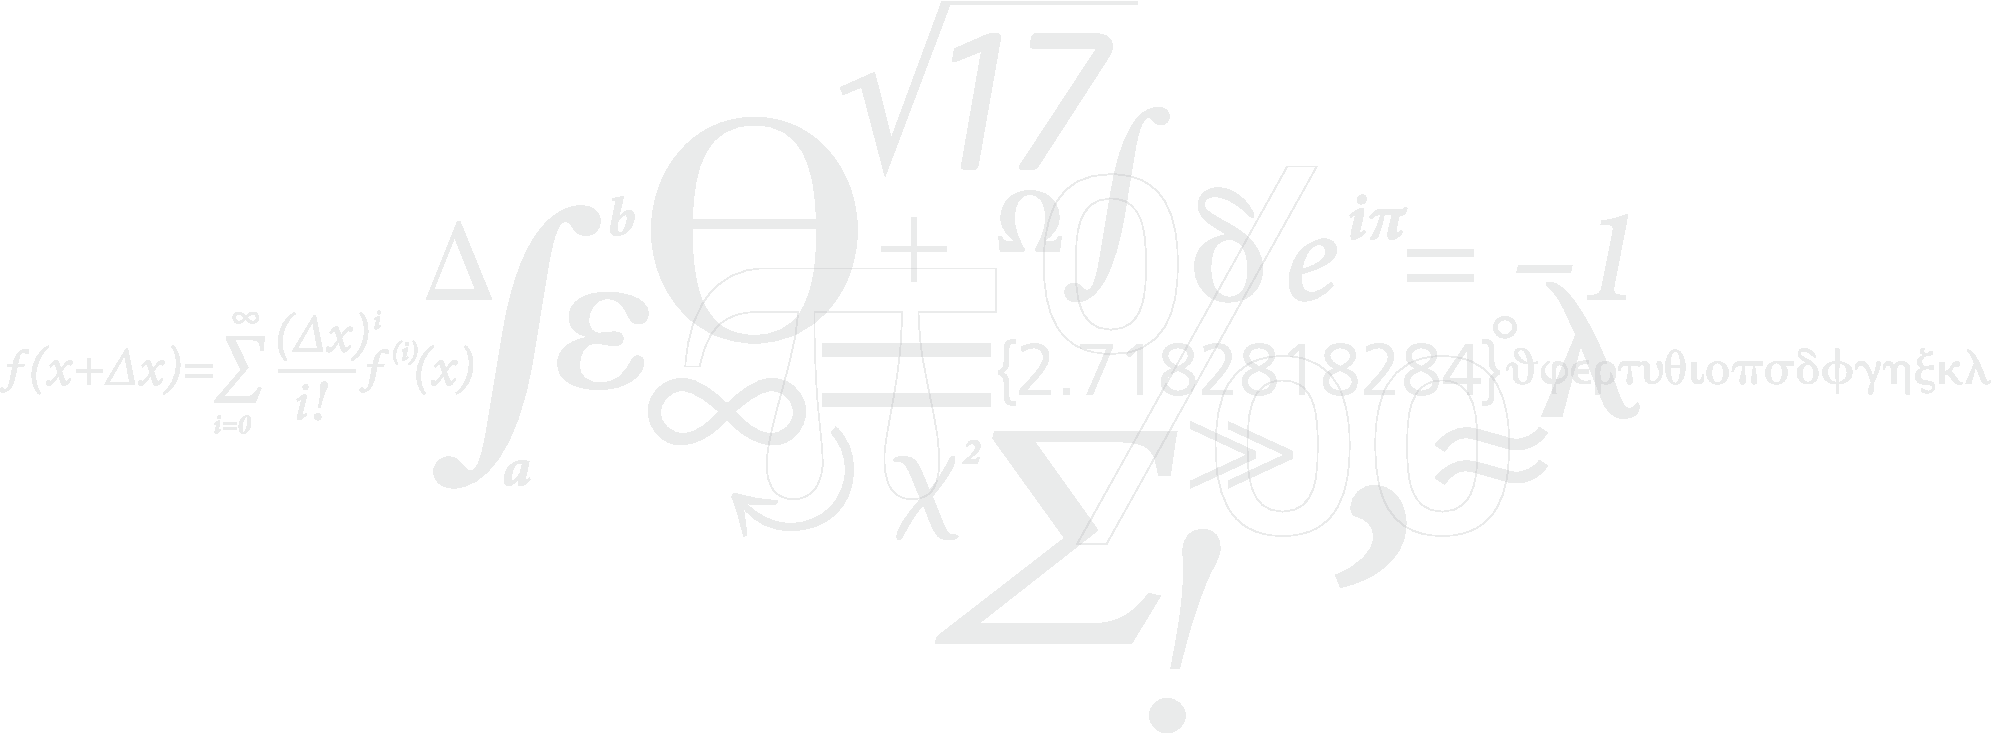
\includegraphics[trim=125mm 0 0 0, clip=true, width=0.66\paperwidth]{figures/DTU-frise-SH-15.pdf}
				\vspace*{1cm}
			}
		}
	}
}
